\subsection{牛顿方法}

\subsubsection{牛顿方法的思路}
\begin{enumerate}
	\item 先介绍如何使用牛顿方法得到某函数的零点,因为在极值点的导数为0,因此,可以用牛顿方法找到导数为0的点,这个点有可能就是个极值点\footnote{这就是不论我们要找的是最大值还是最小值,最终的式子都是一样的原因。}。
	\item 说明
	\begin{enumerate}
		\item 后续在介绍牛顿方法时,仍旧使用逻辑回归作为例子,所以,其似然函数$l(\theta)$还是与逻辑回归一样
	\end{enumerate}
\end{enumerate}

\subsubsection{牛顿方法讲解}
\begin{enumerate}
	\item 牛顿方法介绍: 如下面示意图所示,我们要求的是曲线$y=f(x)$与直线$y=y_{final}$\footnote{若$y_{final}=0$求的就是零点了}的交点$(x_{final}, y_{final})$的值,为此,我们先任取曲线上的一点$(x_{ori}, y_{ori})$,求得在该点的切线,记为$y=f'(x_{ori})x + b$,然后得到该切线与$y=y_{final}$的交点$(x_{new}, y_{final})$,得到$x_{new}$后,我们又可以得到曲线上新的一点$(x_{new}, f(x_{new}))$\footnote{此处写得比较简陋,若不明白建议去看讲义或视频};用新的点$(x_{new}, f(x_{new}))$代替之前的$(x_{ori}, y_{ori})$,重复之前的步骤\footnote{示意图: \url{https://upload.wikimedia.org/wikipedia/commons/e/e0/NewtonIteration_Ani.gif}}。就这样,多次重复后,我们就能逼近我们所要的$(x_{final}, y_{final})$了。
	\begin{figure}[htbp]
		\centering
		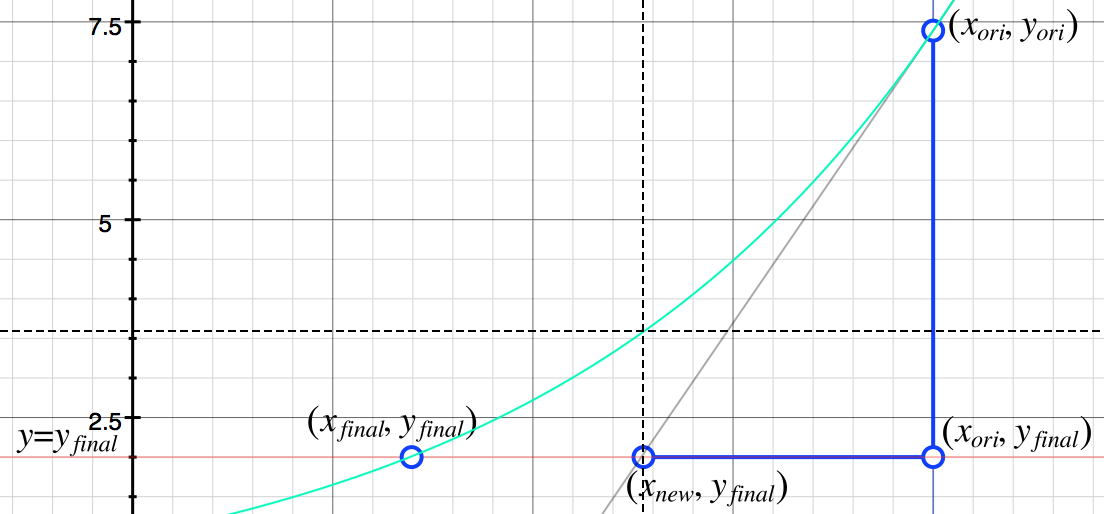
\includegraphics[scale=0.5]{./images/牛顿方法示例图片}
		\caption{牛顿方法示例图}
	\end{figure}

	\item 在逻辑回归中使用牛顿方法的过程
	\begin{enumerate}
		\item 由上图可知,$\tan\alpha = \frac{y_{ori}-y_{final}}{x_{ori}-x_{new}} = \frac{f(x_{ori})-f(x_{final})}{x_{ori}-x_{new}} = f'(x_{ori})$\footnote{$\alpha$是切线$y=f'(x_{ori})x + b$与水平线$y=y_{final}$的夹角,不好标就没画出来了},可以得到
		\begin{equation}
			x_{new} := x_{ori} - \frac{f(x_{ori})-f(x_{final})}{f'(x_{ori})}
		\end{equation}
		
		\item 此时,我们得到了一个新的点$(x_{new}, y_{new})$,相比与原来的点$(x_{ori},y_{ori})$,这个点离最终的$(x_{final}, y_{final})$更近了。

		\item 特殊地,在逻辑回归中,我们要得到的是似然函数$l(\theta)$的极值,极值点的导数为$0$。于是,为了在逻辑回归中使用牛顿方法,我们用$l'(\theta)$代替$f(x)$,且$l'(\theta_{final}) = 0$,于是,上式变成
		\begin{align}
			\theta_{new} &:= \theta_{ori} - \frac{l'(\theta_{ori})-l'(\theta_{final})}{l''(\theta_{ori})} \\
			&:=  \theta_{ori} - \frac{l'(\theta_{ori})}{l''(\theta_{ori})}
		\end{align}
		这就是逻辑回归使用牛顿方法时的迭代方式
	\end{enumerate}

	\item 矩阵表达形式 \\
	将上面的式子改写为矩阵表达的形式,如下
	\begin{equation}
		\theta := \theta - H^{-1}\nabla_{\theta}l(\theta)
	\end{equation}
	其中,$H$称为Hessian\footnote{关于Hessian矩阵的介绍请见附录},是一个$n*n$矩阵
	\begin{equation}
		H_{ij} = \frac{\partial^2l(\theta)}{\partial\theta_i\partial\theta_j}
	\end{equation}

	\item 关于牛顿方法的思考
	\begin{enumerate}
		\item 因为不论我们要得到的是最大值还是最小值,其极值点的导数均为$0$,因此,虽然上述逻辑回归中,我们要得到的时似然函数的极大值,但是,若在其他问题中我们要的得到的时极小值,最终的迭代方式还是一样的。
		\item 但是,通过此方法找到的只是极值点(且每次应该只能找到一个解),很可能只是局部最优,如何保证其为全局最优(最大或最小)呢?。{\color{red}{此项待研究。。}}
	\end{enumerate}

	\item 牛顿方法与梯度下降方法的异同
	\begin{enumerate}
		\item 牛顿方法可以在很少的迭代次数就收敛,而梯度下降要收敛需要迭代的次数可能较多
		\item 但是,牛顿方法每次迭代的计算量较大(因为要计算$H^{-1}$),这在特征维度$n$较大时将会耗费较多的性能
		\item 综上,在特征维度$n$不是太大时,使用牛顿方法能够很快就收敛;但是若特征维度$n$很大时,虽然使用牛顿方法需要迭代的次数较少,但是它每次耗费的计算量太大,整个学习的时间不一定能够比梯度下降少。
	\end{enumerate}
\end{enumerate}














